\documentclass[output=paper,colorlinks,citecolor=brown,
% hidelinks,
% showindex
]{langscibook}
\author{Ernesto R. Guti\'errez Topete\affiliation{University of California, Berkeley}}
\title{Lexical effects on place of articulation of voiced coronal stops of Spanish--English bilinguals}
\abstract{The present study investigates whether bilingual speakers produce one or two phonetic categories for coronal stops in Spanish (L1) and English (L2) speech, given that Spanish is characterized as exhibiting dental stops, whereas English is generally described as having alveolar productions. Under a usage-based framework, I further examine lexical effects of frequency, cognate status, and the lexicon associated with the speakers’ community of practice (i.e. the technology industry), as possible factors that mediate the development of an equivalent but distinct phonetic category in their L2 sound system. I report that the acoustic cues (center  of gravity, standard deviation, skewness, kurtosis, relative intensity) indicate the existence of distinct phonetic categories for Spanish and English, and furthermore, the technology lexicon may drive this development, since English IT words are more alveolar-like than English non-IT words. This study explores novel approaches to remote data collection and to the study of language frequency. \\
 \textit{Keywords}: coronal stops, Spanish--English bilinguals, spectral measurements, relative intensity, Community of Practice-Specific lexicon.}

\IfFileExists{../localcommands.tex}{%hack to check whether this is being compiled as part of a collection or standalone
   % add all extra packages you need to load to this file

\usepackage{tabularx,multicol,multirow}
\usepackage{url}
\urlstyle{same}

\usepackage{listings}
\lstset{basicstyle=\ttfamily,tabsize=2,breaklines=true}

\usepackage{langsci-basic}
\usepackage{langsci-optional}
\usepackage{langsci-lgr}
\usepackage{langsci-gb4e}
%    \let\eachwordone=\it % Ch 14, 18

\usepackage{jambox}
\usepackage{subfigure}
\usepackage{tablefootnote}
\usepackage[nameinlink, noabbrev]{cleveref}
\crefname{enumi}{example}{examples}

\usepackage{bbding}
%\usepackage{linguex}
\usepackage{stmaryrd}

\usepackage{tipa}
\let\ipa\textipa
\usepackage{vowel}
\newcommand{\BlankCell}{}
\usepackage{ot-tableau}

\usepackage{forest}
\useforestlibrary{linguistics}
\usepackage[noeepic]{qtree}
\usepackage{pstricks, pst-xkey, pst-jtree}
\usepackage{tikz-qtree}
\usepackage{tikz-qtree-compat}
\usepackage{tree-dvips}

\usepackage{lastpage}
\usepackage{hyperref}
\usepackage{xltxtra}

\usepackage{ragged2e}
%\usepackage{subcaption}
\usepackage{floatrow}
\usepackage{float}

\usepackage[normalem]{ulem} % Pour les textes barrés
\usepackage{ifthen} 

\usepackage{todonotes}

   \newcommand*{\orcid}{}

\makeatletter
\let\theauthor\@author
\makeatother

\papernote{\scriptsize\normalfont
    \theauthor.
    \titleTemp. 
    To appear in: 
    Chad Howe and Pilar Chamorro and Timothy Gupton and Margaret Renwick.
    Theory, Data, and Practice: Selected papers from the 49th Linguistic Symposium on Romance Language
    Berlin: Language Science Press. [preliminary page numbering]
}

% Workaround for subscripts with capital letters
\newcommand{\capsub}[1]{\ensuremath{_\text{#1}}}

% Chapter 10: Table-like presentation within example environment
% classical latin > {*}late latin > old french  earlier > later   gloss
\newcommand{\montanoboxi}[7]{\parbox{2cm}{#1} > {#2}\parbox{2cm}{#3} > \parbox{1.5cm}{\textit{#4}} \parbox{1.2cm}{#5}\ > \parbox{1.2cm}{#6} \parbox{1.5cm}{#7}}
% {*}latin > earlier OF [ipa] > early OF   gloss
\newcommand{\montanoboxii}[6]{{#1}\parbox{1.9cm}{\textit{#2}} > \parbox{1.3cm}{\textit{#3}} \parbox{2cm}{#4} \parbox{2cm}{#5} \parbox{1.9cm}{#6}}

% Chapter 5
\newcommand{\redc}[1]{\textcolor{red}{#1}}
\newcommand{\bluec}[1]{\textcolor{blue}{#1}}
\newcommand{\ajout}[1]{\textcolor{blue}{#1}}
\newcommand{\ajoutplus}[1]{\textcolor{cyan}{#1}}

\newcommand{\hachure}[9]{
% Parametres :
% Coordonnees bas gauche (2 parametres) : (#1,#2)
% Coordonnees haut droit (2 parametres) : (#3,#4)
% Orientation : #5
%   1 : diagonale de pente 1
%  -1 : diagonale de pente -1
%   0 : horizontal
%   2 : vertical
% Nombre de pas horizontaux : #6
% Epaisseur du trait : #7
% Couleur : #8 (ex. green)
% Atténuation couleur : #9 (ex. 30)
\pgfmathsetmacro{\N}{#6-1}
\pgfmathsetmacro{\A}{#1}
\pgfmathsetmacro{\B}{#2}
\pgfmathsetmacro{\C}{#3}
\pgfmathsetmacro{\D}{#4}
\pgfmathsetmacro{\I}{(#3-#1)/#6}
\pgfmathsetmacro{\J}{(#4-#2)/#6}
\ifthenelse{\equal{#5}{1}}{
  \foreach \n in {0,...,\N}
    \foreach \m in {0,...,\N}
      {
        \pgfmathsetmacro{\X}{\A + ((0 + \n) * \I)}
        \pgfmathsetmacro{\Y}{\B + ((0 + \m) * \J)}
        \pgfmathsetmacro{\U}{\A + ((1 + \n) * \I)}
        \pgfmathsetmacro{\V}{\B + ((1 + \m) * \J)}
        \draw[#8!#9,#7] (\X, \Y)--(\U, \V);
      } 
  }{}
\ifthenelse{\equal{#5}{-1}}{
  \foreach \n in {0,...,\N}
    \foreach \m in {0,...,\N}
      {
        \pgfmathsetmacro{\X}{\A + ((1 + \n) * \I)}
        \pgfmathsetmacro{\Y}{\B + ((0 + \m) * \J)}
        \pgfmathsetmacro{\U}{\A + ((0 + \n) * \I)}
        \pgfmathsetmacro{\V}{\B + ((1 + \m) * \J)}
        \draw[#8!#9,#7] (\X, \Y)--(\U, \V);
      } 
  }{}
\ifthenelse{\equal{#5}{0}}{
  \foreach \n in {0,...,\N}
    \foreach \m in {0,...,\N}
      {
        \pgfmathsetmacro{\X}{\A + ((0 + \n) * \I)}
        \pgfmathsetmacro{\Y}{\B + ((0 + \m) * \J)}
        \pgfmathsetmacro{\U}{\A + ((1 + \n) * \I)}
        \pgfmathsetmacro{\V}{\B + ((0 + \m) * \J)}
        \draw[#8!#9,#7] (\X, \Y)--(\U, \V);
      } 
  }{}
\ifthenelse{\equal{#5}{2}}{
  \foreach \n in {0,...,\N}
    \foreach \m in {0,...,\N}
      {
        \pgfmathsetmacro{\X}{\A + ((0 + \n) * \I)}
        \pgfmathsetmacro{\Y}{\B + ((0 + \m) * \J)}
        \pgfmathsetmacro{\U}{\A + ((0 + \n) * \I)}
        \pgfmathsetmacro{\V}{\B + ((1 + \m) * \J)}
        \draw[#8!#9,#7] (\X, \Y)--(\U, \V);
      } 
  }{}
}

%Définition d'un pattern de type hachure
% \usetikzlibrary{patterns}
% \makeatletter
% \tikzset{hatch distance/.store in=\hatchdistance,hatch distance=5pt,hatch thickness/.store in=\hatchthickness,hatch thickness=5pt}

% \pgfdeclarepatternformonly[\hatchdistance,\hatchthickness]{north east hatch}% name
%     {\pgfqpoint{-\hatchthickness}{-\hatchthickness}}% below left
%     {\pgfqpoint{\hatchdistance+\hatchthickness}{\hatchdistance+\hatchthickness}}% above right
%     {\pgfpoint{\hatchdistance}{\hatchdistance}}%
%     {
%         \pgfsetcolor{\tikz@pattern@color}
%         \pgfsetlinewidth{\hatchthickness}
%         \pgfpathmoveto{\pgfqpoint{-\hatchthickness}{-\hatchthickness}}       
%         \pgfpathlineto{\pgfqpoint{\hatchdistance+\hatchthickness}{\hatchdistance+\hatchthickness}}
%         \pgfusepath{stroke}
%     }
% \pgfdeclarepatternformonly[\hatchdistance,\hatchthickness]{north west hatch}% name
%     {\pgfqpoint{-\hatchthickness}{-\hatchthickness}}% below left
%     {\pgfqpoint{\hatchdistance+\hatchthickness}{\hatchdistance+\hatchthickness}}% above right
%     {\pgfpoint{\hatchdistance}{\hatchdistance}}%
%     {
%         \pgfsetcolor{\tikz@pattern@color}
%         \pgfsetlinewidth{\hatchthickness}
%         \pgfpathmoveto{\pgfqpoint{\hatchdistance+\hatchthickness}{-\hatchthickness}}
%         \pgfpathlineto{\pgfqpoint{-\hatchthickness}{\hatchdistance+\hatchthickness}}
%         \pgfusepath{stroke}
%     }
% \makeatother
%~~~~~~~~~~~~~~~~~~~~~~~~~~~~~~~~~~~~~


% Chapter 7
\newcommand\pef[1]{(\ref{#1})}

\newcommand{\subscript}[1]{\textsubscript}

   %% hyphenation points for line breaks
%% Normally, automatic hyphenation in LaTeX is very good
%% If a word is mis-hyphenated, add it to this file
%%
%% add information to TeX file before \begin{document} with:
%% %% hyphenation points for line breaks
%% Normally, automatic hyphenation in LaTeX is very good
%% If a word is mis-hyphenated, add it to this file
%%
%% add information to TeX file before \begin{document} with:
%% %% hyphenation points for line breaks
%% Normally, automatic hyphenation in LaTeX is very good
%% If a word is mis-hyphenated, add it to this file
%%
%% add information to TeX file before \begin{document} with:
%% \include{localhyphenation}
\hyphenation{
anaph-o-ra
Dor-drecht
%FFI2016-76045-P-AEI/-MINEICO/-FEDE
}

\hyphenation{
anaph-o-ra
Dor-drecht
%FFI2016-76045-P-AEI/-MINEICO/-FEDE
}

\hyphenation{
anaph-o-ra
Dor-drecht
%FFI2016-76045-P-AEI/-MINEICO/-FEDE
}

    \bibliography{localbibliography}
    \togglepaper[23]
}{}

\begin{document}
\maketitle

\section{Introduction}

Phonetic variation in language has been linked to different linguistic, social, and usage-based factors \citep{labov1994principles,labov2001principles,bybee2001phonology,pierrehumbert2001exemplar}, which for Spanish have been most notably established through the study of the reduction of /s/ (see \citealp{brown2008usage} for a general overview of the literature). The production of coronal stops by Spanish--English bilinguals, however, represents the pairing of a feature and a population that have received less attention in the field. This feature is of particular interest because of its characteristic differences between the two languages: while monolingual Spanish is described as having a single coronal stop category, dental /d̪/ \citep{hualde2005sounds}, most varieties of English are characterized by an alveolar /d/ \citep{hammond1999phonology}. Yet, the articulation of this sound by Spanish--English bilingual speakers remains remarkably understudied. I purposefully examine language production by an equally unexplored population of bilingual speakers: Mexican residents who use English at work in the information technology (IT) industry.

In the present study, I investigate the acoustic properties of word-inital /d/ in Spanish and English speech, as produced by early Spanish--English bilingual speakers. I uniquely analyze a combination of four spectral moments, namely center of gravity, standard deviation, skewness, and kurtosis, as well as relative intensity. In so doing, I examine which metrics best characterize variation in /d/ production. The population studied here is composed of Spanish--L1--English--L2 IT workers in Mexico who primarily use English in the workplace, while Spanish is predominant in their daily life outside of work. The main motivation for the present study is to investigate whether Spanish--English bilingual speakers display one or two (i.e. dental and/or alveolar) phonetic articulations in their Spanish and English speech. Following usage-based models of language variation, I further investigate whether or not factors such as general frequency, community of practice (specifically, IT) status, and cognate status of the words where the phones are produced mediate the productions of these sounds. Lastly, I introduce a new methodology for conducting quality phonetics research remotely, which is becoming increasingly relevant given the current global health crisis.

The present paper is structured in the following way: in \sectref{sec:gutierrez:lit}, I provide acoustic and articulatory characteristics of /d d̪/ variation in English and Spanish and discuss social and linguistic factors under consideration. I also review usage-based models and exemplar theory of language representation, which I use to ground my research question and hypotheses. Lastly, I provide an argumentation in favor of Community of Practice-Specific lexicon in the study of language variation. \sectref{sec:gutierrez:study} describes the present study, including an innovative methodology that may be used for remote data collection for phonetic studies. Then, \sectref{sec:gutierrez:results} provides the results obtained in this study. Finally, \sectref{sec:gutierrez:discussion} contains a discussion of the results and novel approaches advocated for in this paper, and \sectref{sec:gutierrez:conclusion} concludes with specific and general linguistic implications from this study.

\section{Phonetic variation}\label{sec:gutierrez:lit}

Starting with Labov's fundamental studies of New York speech during the mid 20\textsuperscript{th} century \citep{labov1963social,labov1966social}, the effects of linguistic, social, and usage-based factors have been mapped onto the production of language. The production of dental or alveolar /d/ by Spanish--English speakers in the present study is no different. Although this variable has its own set of complexities, it is governed by similar constraints (i.e. linguistic, social, and cognitive) as countless other variables demonstrated in the literature.

\subsection{Articulation and acoustics of coronal stops}

Coronal stops in Spanish and English may be distinguished based on place of articulation (\textsc{poa}). For instance, in American English, coronal stops are generally characterized as alveolar \citep[see \figref{fig:gutierrez:cor_alv}]{hammond1999phonology}. Some speakers of subdialects of American English such as New York English and African American Vernacular English have also been reported to produce interdental fricatives as dental stops \citep{gordon2008new,green2002african}. Contrastively, Spanish is typically described as having a dental articulation of coronal stops \citep[see \figref{fig:gutierrez:cor_den}]{hualde2005sounds}. Furthermore, in intervocalic position, the production of the voiced coronal stop in Spanish is most commonly a voiced approximant [ð]. This allophonic variation occurs mainly in word-medial position or in running speech where the coronal sounds, either in word-inital or word-final position, are found in an intervocalic environment. Furthermore, voice onset time (\textsc{vot}), the start of glottal vibrations in the production of plosives, is also said to differ between the two languages; whereas voiced coronal stops in English have a short \textsc{vot} lag (i.e. vibrations begin after the release burst), /d/ in Spanish typically has a \textsc{vot} lead (i.e. glottal vibrations begin prior to the release of the burst;)\citep{lisker1964cross,keating1984phonetic}.

\begin{figure}
    \subfigure[ Alveolar stop]{{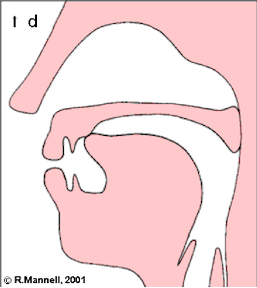
\includegraphics[width=5cm]{figures/gutierrez_cor_alv.png} \label{fig:gutierrez:cor_alv} }}%
    \qquad
    \subfigure[ Dental stop]{{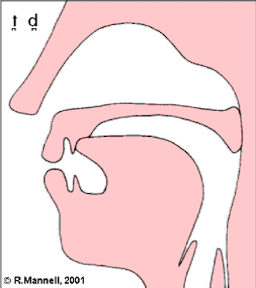
\includegraphics[width=5cm]{figures/gutierrez_cor_den.png} \label{fig:gutierrez:cor_den} }}%
    \caption{Coronal stops (images incorporated from \citealt{mannell2001pic})}%
    \label{fig:gutierrez:coronal_stops}%
\end{figure}

In acoustic studies, spectral measurements (i.e. center of gravity (\textsc{cog}), standard deviation (\textsc{sd}), skewness, and kurtosis) and relative intensity (\textsc{ri}) of burst productions have been found to correlate with \textsc{poa} of coronal stops; that is, values of these properties vary based on the constriction location of the phone \citep{jongman1985acoustic,sundara2005acoustic,sundara2006production,sundara2008discrimination}. Whereas the spectral measurements -- or moments -- measure the energy distribution across frequency bands in the signal, intensity represents the power and loudness of a sound. Studies that explored the aforementioned metrics in languages with dental or alveolar stops -- or both -- have found patterns in the acoustic measurements of interest, with consistent trends. In other words, \textsc{cog}, \textsc{sd}, skewness, kurtosis, and \textsc{ri} values differ for dental and alveolar stops in the same way, cross-linguistically, signaling that they are correlated with \textsc{poa}.

To my knowledge, \citet*{casillas2015acoustics} are the only researchers to look into acoustic differences between English alveolar and Spanish dental stops. The researchers compared acoustic properties of the production of monolingual Spanish and English speakers. However, the authors only analyzed English /d/ and Spanish /t/, in order to control for \textsc{vot} differences, as both sounds are typically realized with a short lag. In this specific study, they found that there were differences in \textsc{cog}, \textsc{sd}, and \textsc{ri} as a function of language (i.e. \textsc{poa}). \textsc{cog} results corroborate the findings by other researchers, but \textsc{ri} and \textsc{sd} values contradict them. Note that \citeauthor{casillas2015acoustics} examined voiced /d/ and voiceless /t̪/; thus, it is possible that comparing two phonemes with distinct voicing categories may result in such discrepancies. The articulatory behavior of Spanish--English bilinguals in regard to the production of coronal stops, nonetheless, remains unexplored. Thus, the study of the aforementioned acoustic cues may inform us about the articulatory production of coronal stops by bilingual speakers whose languages distinguish between alveolar and dental stops.

\subsection{Usage-based models of language variation}

Usage-based models of language \citep[e.g.][]{bybee2001phonology,pierrehumbert2001exemplar} propose that there is a close connection between the mental representation of language and its usage. The models suggest that there is a reciprocal influence between the two: ``usage feeds into the creation of grammar just as much as grammar determines the shape of usage'' \citep[730]{bybee2006usage}. This means that, in the domain of phonetics and phonology, ``language use plays a role in shaping the form and content of sound systems'' \citep[1]{bybee2001phonology}. Drawing from exemplar theory of phonetic categories \citep{johnson1997speech}, the models further postulate that language users will store exemplars or instances of each linguistic item they are exposed to in their memory, in addition to the contextual information in which the token was produced (e.g. speaker's characteristics, linguistic and social context, etc.). These exemplars are later categorized in clouds of closely related exemplars, and the quintessential representation of a word or sound will be the most frequent linguistic item represented in the cloud. Less frequent items are often stored on the periphery of these exemplar clouds, which makes them more difficult to activate and retrieve during language production, relative to more frequent tokens.

In addition, these models are also able to account for the different patterns observed for certain words. It was first reported as early as the 19\textsuperscript{th} century that not all words follow sound variation and change at the same rate or even to completion \citep{schuchardt1885lautgesetze}. The irregular path in the application of sound changes followed by certain words, when compared to peer words with the same sound, has been attested in a myriad of cases and was denominated \textit{lexical diffusion} \citep{phillips1984word,phillips1999mental,bybee2000phonology}. In phonetically-motivated sound changes, it is more likely that a sound change will be completed (at a faster pace) in frequent than infrequent words. This empirical evidence is a strong indication that exposure to language influences language representation and production patterns.

Considering the postulates stated above, usage-based models require a great deal of labor in storing all these exemplars in an individual's memory (see \citeauthor[140]{pierrehumbert2001exemplar} for further discussion). However, the process of language production, as stipulated in these models, becomes straightforward and simple, if it is based on experiential memory and associated levels of activation. These models are well equipped to account for phonetic differences linked to the usage -- and thus, frequency -- of words. Another strength of these models is related to the additional extralinguistic information stored in conjunction with the linguistic information of each exemplar. Exemplar theory and usage-based models argue that listeners store information about the speaker who produced the linguistic item and the context in which it was uttered. As such, the environment and the group of people with whom an individual interacts on a regular basis (i.e. the community of practice) will affect the propagation of sound changes.

\subsection{Social factors: community of practice}

As initially described by Gumperz, the \textit{speech community} is ``[a] social group which may be either monolingual or multilingual, held together by frequency of social interaction and set off from the surrounding areas by weaknesses in the lines of communication'' \citep[101]{gumperz1971language}. That is, the group of interest and reference for sociolinguistic research, given Gumperz's argumentation, should be a group of speakers who interact frequently with one another, more so than with members of other groups. Furthermore, Labov narrows down this definition making reference to social norms: 

\begin{quote}
The speech community is not defined by any marked agreement in the use of language elements, so much as by participation in a set of shared norms: these norms may be observed in overt types of evaluative behavior, and by the uniformity of abstract patterns of variation which are invariant in respect to particular levels of usage. \citep[120--1]{labov1972sociolinguistic}

\end{quote}

\noindent In sum, a speech community is a group of individuals with frequent and constant communication, with specific social norms and orderly heterogeneity in regard to language use.


Going beyond the speech community to explain linguistic behavior in social settings, \citet{holmes1999community} provide a theoretical basis within sociolinguistics for the term \textit{community of practice}. As originally introduced by \citet{eckert1992think}, a community of practice (CofP) is:

\begin{quote}
    An aggregate of people who come together around mutual engagement in an endeavor. Ways of doing things, ways of talking, beliefs, values, power relations -- in short, practices -- emerge in the course of this mutual endeavor. As a social construct, a CofP is different from the traditional community, primarily because it is defined simultaneously by its membership and by the practice in which that membership engages. (\citeyear[464]{eckert1992think})
\end{quote}

\noindent This definition dives deeper into the community and its membership, and it highlights the importance of ``practice." Furthermore, drawing from \citeauthor{wenger1998communities}'s (\citeyear{wenger1998communities}) argumentation of learning in social contexts, \citeauthor{holmes1999community} state that:

\begin{quote}
    The process of becoming a member of a CofP -- as when we join a new workplace, a book group, or a new family (e.g. through marriage) -- involves learning. We learn to perform appropriately in a CofP as befits our membership status: initially as a `peripheral member,' later perhaps as a `core member' (or perhaps not -- one may choose to remain a peripheral member). In other words, a CofP inevitably involves the acquisition of sociolinguistic competence. (\citeyear[174]{holmes1999community})
\end{quote}

\noindent The appeal of this re-examination of the social groups -- with a focus on what members do, given the social learning that has taken place -- provides us with a framework to analyze how joining a new social group and becoming a practicing member may be manifested in the process of learning about and gaining control of the language appropriate for that practice \citep[175]{holmes1999community}.

Some recent studies \citep[e.g.][]{file2011gradient,erker2012role,linford2013lexical} have adopted practices for the measurement of lexical frequency at a `local' level. For instance, \citeauthor{file2011gradient} used (local) lexical frequencies observed in the same corpus from which the data were collected for the study of /s/ reduction in Cale{\~n}o Spanish. Nonetheless, the tradition in the field, and in particular in psycholinguistics, as expressed by \citet{brysbaert2009moving}, has been to use the general lexical frequencies in works such as \citet{kucera1967computational} (see \citealt{burgess1998effect} and \citealt{erker2012role} for similar critiques). The criticisms of such a practice have questioned the relevance of population-general lexical frequencies in the linguistic behavior of specific communities. 

Accordingly, in this paper I argue for the study of Community of Practice-Specific (CPS) lexicon and lexical frequency, an approach that analyzes and compares the behavior of a social group linked by a particular practice to the group itself. CPS lexicon refers to those words used with heightened frequency in a given community that engages in a particular practice. This lexicon may be associated to hobbies or interests, habitual activities, or daily responsibilities. By definition, CPS lexicon needs to exist within a social group (i.e. the community of practice), thus ensuring that members have plenty of exposure to and practice producing these words. Some examples of CPS lexicon are those terms such as \textit{revenue} and \textit{accruals} used by professional accountants or \textit{diaper} and \textit{stroller} used by and between new parents. 

Guided by empirical evidence and usage-based models, I propose that CPS lexicon is a more valid representation of lexical frequency, given that these words are encountered more frequently within the community in question. If a given word is used frequently in a particular community, members of that community should show frequency effects. However, these effects should not be expected to be manifested in non-members of this community of practice -- or not to the same degree -- given that those individuals quite possibly subscribe to other social practices, and thus display linguistic behaviors appropriate to their respective communities of practice.

\subsection{Linguistic factors: lexical frequency and cognate effects}

Ample research in phonetic variation has shown that the studied phenomena are governed by social, cognitive and linguistic factors -- linguistic factors such as lexical frequency and cognate status. As discussed to some extent in the previous sections, lexical frequency has intervening effects in phonetic variation. For instance, sound changes affect high-frequency and low-frequency words disproportionately, as exemplified by cases of lexical diffusion \citep{schuchardt1885lautgesetze,phillips1984word,phillips1999mental,bybee2000phonology}. Current usage-based models of language representation argue that these lexical frequency effects are due to the high representation, and thus activation, of more frequent linguistic items. Therefore, it is expected that lexical frequency effects will manifest themselves in linguistic productions of high- vs. low-frequency words in phonetic variation cases.

In addition to frequency effects, cognate status has been found to play a role in phonetic variation. Cognates are words in two languages that share both semantic and phonological similarities (e.g. \emph{television} and \emph{televisi{\'o}n} in English and Spanish, respectively). Non-cognate words, on the other hand, are translation equivalents with distinct phonological forms (e.g. \emph{tree} in English and \emph{{\'a}rbol} in Spanish). Cognate status, as reported by \citet{amengual2012interlingual}, for instance, has a particular effect in bilingual speech. In his study, \citeauthor{amengual2012interlingual} found that in Spanish, Spanish--English bilinguals of different fluency levels produced Spanish words with English cognates with \textsc{vot} values that were more English-like than their non-cognate counterpart. In a follow-up study, the researcher also found that advanced Catalan--Spanish bilinguals had lower accuracy in a production and lexical decision task that examined the Catalan--Spanish back mid-vowel distinction /o $\sim$ ɔ/ in cognate pairs \citep{amengual2016cross}.

In reviewing different studies of the cognate effect, \citet{costa2005facilitatory} conclude that, ``at present, the most parsimonious way to account for the cognate benefits in speech production is by assuming the existence of interactivity between the lexical and sublexical levels of representation, both within and across the two languages of a bilingual speaker'' (101). Such a conclusion provides an explanation that accounts for the results of phonetic production research. That is to say, in cognate pairs, the activation of a lexical item in one language will activate the corresponding item in the other; both will then activate the phonological segments for those words in both languages, as well as their corresponding phonetic features. It is, then, expected that phonetic features of one language manifest themselves in the production of an equivalent phoneme in the other language for cognate pairs.

\section{The present study}\label{sec:gutierrez:study}

In the present study, I investigate lexical effects on the production of coronal stops in a word list reading task. This study examines the production of the voiced /d/ by early Spanish--English bilinguals working in the IT industry in Mexico, who have Spanish as their L1 and English as their L2. In accordance with the models of language representation described above, I investigate which factors mediate the productions of the voiced coronal stop as either [d] or [d̪]. Consequently, participants read aloud from a list of 93 unstressed /d/-initial words that are controlled for language (Spanish, English), lexical frequency (high, low), CPS status (IT, non-IT vocabulary), as well as cognate status (cognate, non-cognate). Given the reported differences in acoustic cues of dental and alveolar stops, I hypothesize that if these bilinguals have two phonetic categories, they will display a distinction in the acoustic properties in the production data of both languages. I further presume that the difference will be greater in IT lexicon and non-cognate words; the former will results from effects due to increased frequency, and the latter will result from lower levels of cross-linguistic interference, relative to their cognate counterparts.


\subsection{Participants}

For this study, I recorded the speech of 11 early Spanish--L1--English--L2 bilinguals (see \tabref{tab:gutierrez:participant_general} for a breakdown of participant characteristics). The participants (4 females, 7 males) were all born and raised in Mexico. At the time of recording, all participants lived in predominantly Spanish-speaking communities: Mexico City and Guadalajara. All speakers worked for the technology industry in Mexico, a sector where knowledge of English is essential. All but one of the participants started learning English at or before the age of six, through private schooling in Mexico.

\begin{table}
\caption{Summary of participant information}
\label{tab:gutierrez:participant_general}
 \begin{tabular}{lrrr}
 \lsptoprule
 & Range & Mean & \textsc{sd} \\
 \midrule
 Age & 24.4--44.4 & 30.9 & 6.3 \\
 Age of acquisition (Eng) & 3--13 & 5.4 & 2.9 \\
 Years in Eng-speaking workplace & 1--12 & 5.4 & 3.9 \\
 Lang use at work (Eng) & 30\%--95\% & 55.8\% & 19.6\% \\
 \lspbottomrule
 \end{tabular}
\end{table}

Because this study examines general lexical frequency and CPS status, it was essential to examine a group of bilingual speakers with a specialized terminology. Ultimately, this group of bilinguals was chosen for their specific bilingualism, which essentially is isoglossic: professional bilingualism. At work, they are immersed in an English-dominant environment, and outside of work, they interact with people primarily in Spanish. Given that for people in the IT industry (a) knowledge of English is required to learn how to program, due to the nature of coding languages; (b) international communications with other companies or offices worldwide is frequent; and (c) international employment transfers are commonplace, English has become the universal language within the industry. This particular group of bilinguals is in constant communication with native American English speakers who work in the Mexico offices or with native American English speakers who work at the company's headquarters located in California's Bay Area; this communication revolves around IT language (i.e. CPS lexicon). Contrastively, when they leave work at the end of the day, they enter a Spanish-dominant environment in their respective cities (Mexico City and Guadalajara). Therefore, this nearly isoglossic language context provides a perfect opportunity to study potential effects of general lexical frequency and CPS lexicon within IT. Their Spanish knowledge is diverse and general, whereas their English lexicon is IT profession-specific.

\subsection{Materials}

I devised a list of 93 /d/-initial words in Spanish and English. The list was composed of content words (i.e. verbs, nouns, and adjectives), exclusively; differences across grammatical categories were not analyzed in this study. Forty-five words were in English and 58 in Spanish. Forty-eight words were marked as high-frequency, and the other 55 as low-frequency. Finally, 62 words were considered IT lexicon and the remaining 41 were general words. Unstressed /d/-initial tokens were selected for a concordant comparison between the two languages; in Spanish, word-initial stress is rare in words with three or more syllables. The comparable unstressed status between the word lists in the two languages ensured that there were no energy distribution differences at the burst as a result of stress differences. Only unstressed /d/ was used due to the limited number of /t/-initial, unstressed words with these characteristics in English and Spanish. All factors were fully crossed, yielding 16 cells with an average of 6 tokens per cell. One hundred and five fillers were included to mask the sound of interest: /d/. The fillers were unrelated, real words that started with any sound (vowel or consonant) other than /d/. \tabref{tab:gutierrez:stimuli} includes a few sample stimuli in English.

\begin{table}
\caption{Sample English stimuli}
\label{tab:gutierrez:stimuli}
 \begin{tabularx}{\textwidth}{cccccccc}
 \lsptoprule
 \multicolumn{4}{c}{\textsc{cognate}} & \multicolumn{4}{c}{\textsc{non-cognate}} \\ \cmidrule(lr){1-4}\cmidrule(lr){5-8} 
 \multicolumn{2}{c}{\textsc{it}} & \multicolumn{2}{c}{\textsc{non-it}} & \multicolumn{2}{c}{\textsc{it}} & \multicolumn{2}{c}{\textsc{non-it}} \\
 \cmidrule(lr){1-4}\cmidrule(lr){5-8} 
 \textsc{high} & \textsc{low} & \textsc{high} & \textsc{low} & \textsc{high} & \textsc{low} & \textsc{high} & \textsc{low} \\
 %\midrule
 \textit{domain} & \textit{directory} & \textit{decision} & \textit{defoliate} & \textit{device} &  \textit{debug} & \textit{decline} & \textit{debrief} \\
 \lspbottomrule
 \end{tabularx}
\end{table}

For this study, the CPS status (i.e. IT lexicon) was coded based on the words' appearance in online dictionaries or glossaries of programming/coding jargon and/or their appearance as \emph{keywords} listed in online manuals, articles, or websites that provide programming tutorials. Lexical frequency was determined with typical frequency norms, using NIM's Spanish and English corpora \citep{guasch2013nim}. The NIM corpora were used because they include English and Spanish lexical frequencies in a format that has been standardized for straightforward comparisons between the two languages. Each word was labeled as either high- or low-frequency based on their occurrence in these corpora, in order to make a 16-way comparison across the three lexical factors and the two languages; this allowed me to fully cross all factors. The split for high- and low-frequency words was made at the relative frequency (\textsc{rel. f.}) level of 10 parts per million (ppm). High-frequency words had a mean \textsc{rel. f.} of 55.5 ppm, with a standard deviation of 43.6. Their low-frequency counterparts had a mean \textsc{rel. f.} of 2.3 ppm and a standard deviation of 4.1. The difference in \textsc{rel. f.} between high- and low-frequency words was tested in a 1-tailed \textit{t}-test and was found to be significant (\textit{df} = 91, \textit{p}<0.001).

\subsection{Procedures}

The recruitment for this study was initiated via a personal contact and continued using the snowball effect. All subjects participated in an interview conducted over the phone, and they were asked to self-record. Prior to starting the data collection sessions, all subjects were directed to follow strict instructions to undergo a screening process and to prepare for the remote data collection, to ensure quality recordings. The participants were asked to utilize a Mac laptop computer to access all word list materials and to produce the audio recordings; this allowed me to minimize hardware differences in recording equipment across participants. Subjects were also instructed to download the Audacity® software on these computers and were shown how to use basic functions in this program \citep[e.g. recording, stopping, and saving audio recordings as wav files;][]{audacity}. Subjects were also asked to set the sampling frequency to 44100 Hz. Finally, they were told to find an adequate recording location: a room that was not too small and that did not have a lot of exposed, solid wall space, to avoid an echo in the recordings. All participants sent a two-minute sample recording in Spanish prior to the interview session as part of the screening process; these screening samples showed the researcher that all conditions were adequate to produce quality recordings for phonetic analysis: (a) adequate volume, (b) clear speech, (c) clear waveforms and spectrograms, and (d) no echo.

During the interview sessions, each subject received a phone call directly from the researcher. The researcher first confirmed that the participant was fluent in English and Spanish by asking introductory questions in both languages to ensure that they could hold a conversation in both; all participants were able to communicate clearly in English and Spanish. The data collection session, subsequently, continued primarily in Spanish. Shortly after determining bilingual fluency, each participant received a link with a Qualtrics survey \citep{qualtrics}. This survey included a consent form, an attachment with the stimuli list, and a demographic questionnaire. None of the subjects had access to the list of stimuli prior to the recording session. The word list was provided in one single block, and the words were randomized within the block. The block alternated between the two languages, and each word was labeled with the word ``Spanish'' or ``English'' depending on which language needed to be used; this label was added to aid with the production of cognates with (near) identical spelling (e.g. \textit{decision} and \textit{decisi{\'o}n}). This list was presented in a slide show format to ensure participants saw one word at a time and did not have access to upcoming (or previous) stimuli during the reading task. The data collection was composed of a word list reading task and a demographic questionnaire. Only the reading task was audio recorded. At the end of the data collection session, each subject submitted the audio recording to the researcher electronically; questionnaire answers were automatically saved upon submission.

I recognize that a reading task is not the optimal methodology for analyzing speech variation patterns. However, taking into consideration other concerns, which have been previously expressed by \citet{file2009role}, I followed his approach of examining lexical frequency effects in a word list reading task. In particular, \citeauthor{file2009role} indicated that data collection in a naturalistic manner does not provide a fair comparison between low- and high-frequency words: ``[I]nformal conversational speech is characterized by an overall paucity of low-frequency lexical items plus a preponderance of extremely high-frequency items'' (\citeyear[350]{file2009role}). In addition, Spanish /d̪/ is typically produced as an approximant [ð] in intervocalic position, an environment that is more likely to occur in running speech, even to word-initial and -final tokens. For that reason, a reading task with /d/-initial tokens was selected for the analysis of plosive productions.

\subsection{Analysis}

The production data were transcribed as textgrid files using the Praat software \citep{Boersma2009}. The tokens were manually delimited at the word level in the textgrid files and were forced aligned at the phoneme level. While the English data were aligned using the Berkeley Phonetics Machine forced aligner \citep{sprouse2016berkeley}, Spanish data were aligned with faseAlign \citep{wilbanks2018fasealign}. For the data analysis, all audio files were filtered with a stop band filter. This filter had a range between 0 and 300Hz. The stop band filter was applied to eliminate the differences in voicing between Spanish and English voiced coronal stops, given that significantly more prevoicing was present in the Spanish data, albeit also present in English; this ensured that potential differences in the acoustic measures are not the result of voicing discrepancies between the two languages. Moreover, using a Python script which located the approximate time of stop bursts, I retrieved a timestamp of the burst (for a description of this program, see \citealt{lin2019burst}). This program returned the timestamp with the greatest change in Mel-frequency cepstral coefficients (MFCC) per token; this correlated well with the burst release. From each timestamp, a 20ms window of the signal was obtained (5 ms before and 15 ms after the timestamp), and from that window, all five acoustic measures were calculated for the stop productions.

In total, 1,023 tokens were collected through the reading task. From the original list: (a) 47 tokens were thrown out due to poor audio quality, (b) 4 tokens were thrown out because the wrong lexical item was produced, and lastly, (c) 173 tokens were discarded from English and Spanish data because the tokens included the production of an approximant [ð] with no audible or visible burst release. The remaining 799 tokens were included in the analysis of this study. All of these tokens were manually checked for audible and visible signs of a burst in the waveform and the spectrogram on Praat (i.e. a transient and a burst of energy across different frequency bands, respectively). See \figref{fig:gutierrez:declaratory} and \figref{fig:gutierrez:debriefing} for examples of a token with a burst and another without a burst.

\begin{figure}
    
    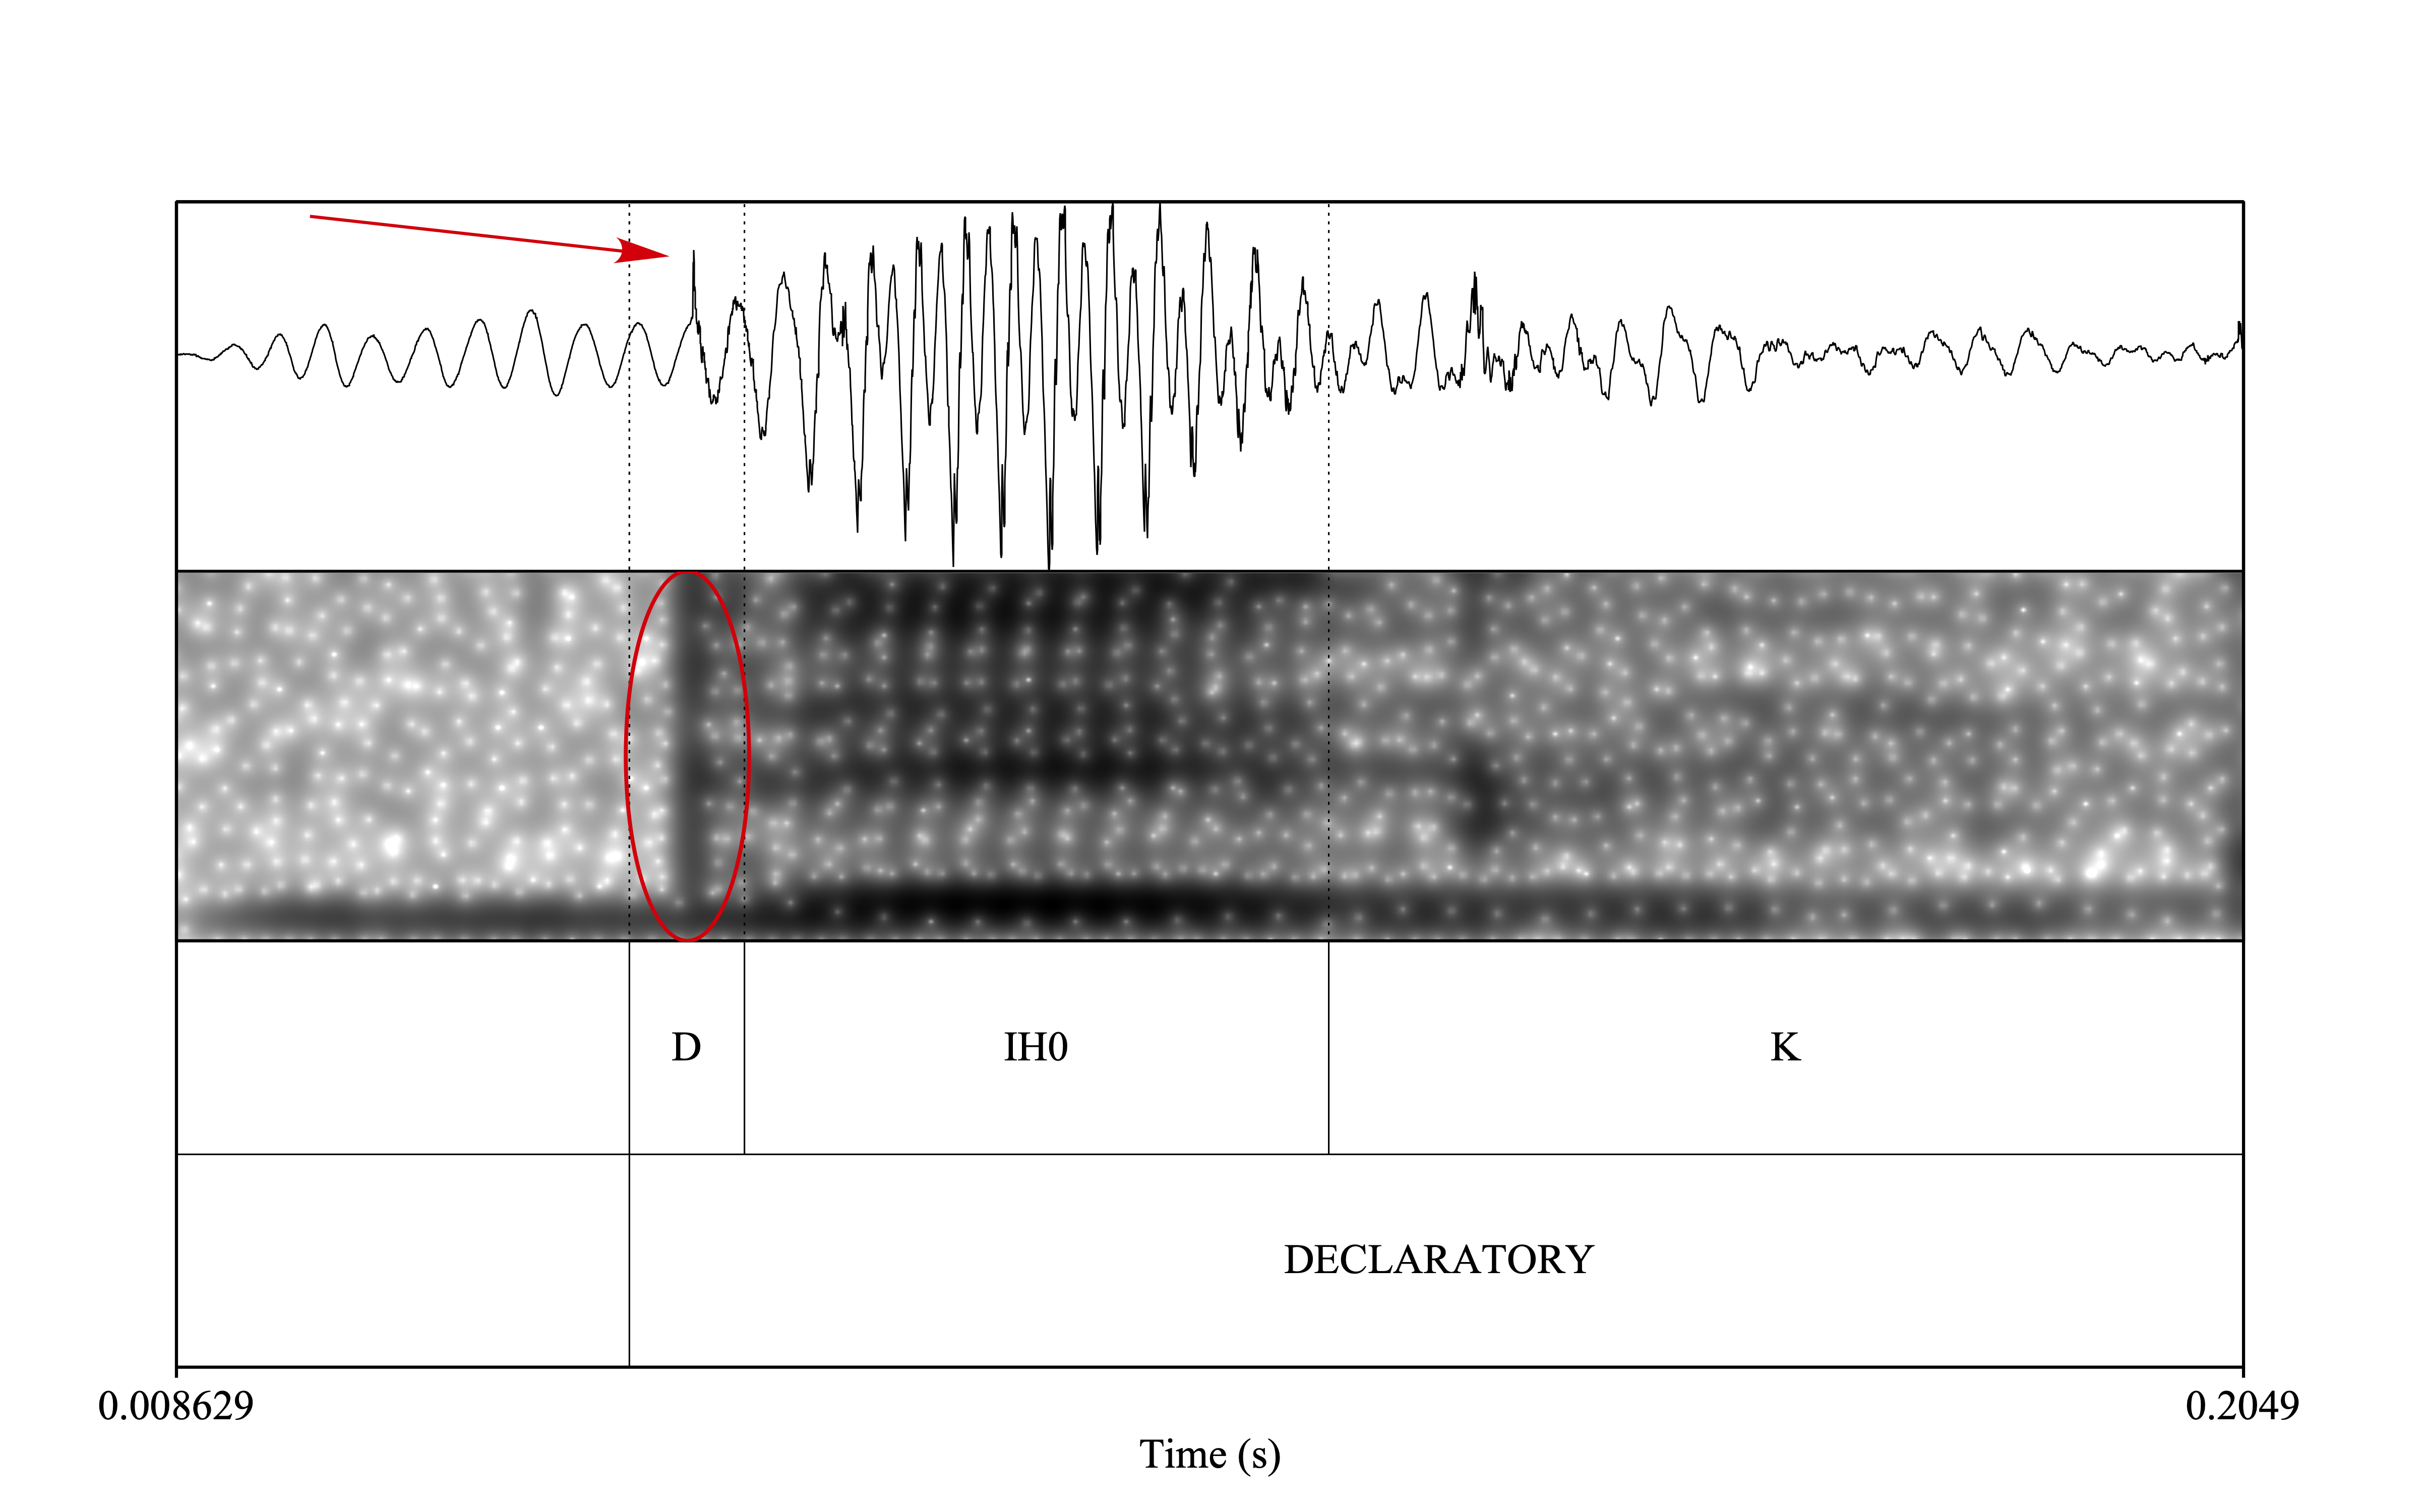
\includegraphics[width=\textwidth]{figures/gutierrez_dec_600.png}
    \caption{A portion of the waveform and spectrogram for the word ``declaratory.'' This image includes a visible burst in the waveform and spectrogram, which are marked by an arrow and an ellipse, respectively.}
    \label{fig:gutierrez:declaratory}
\end{figure}

\begin{figure}
    
    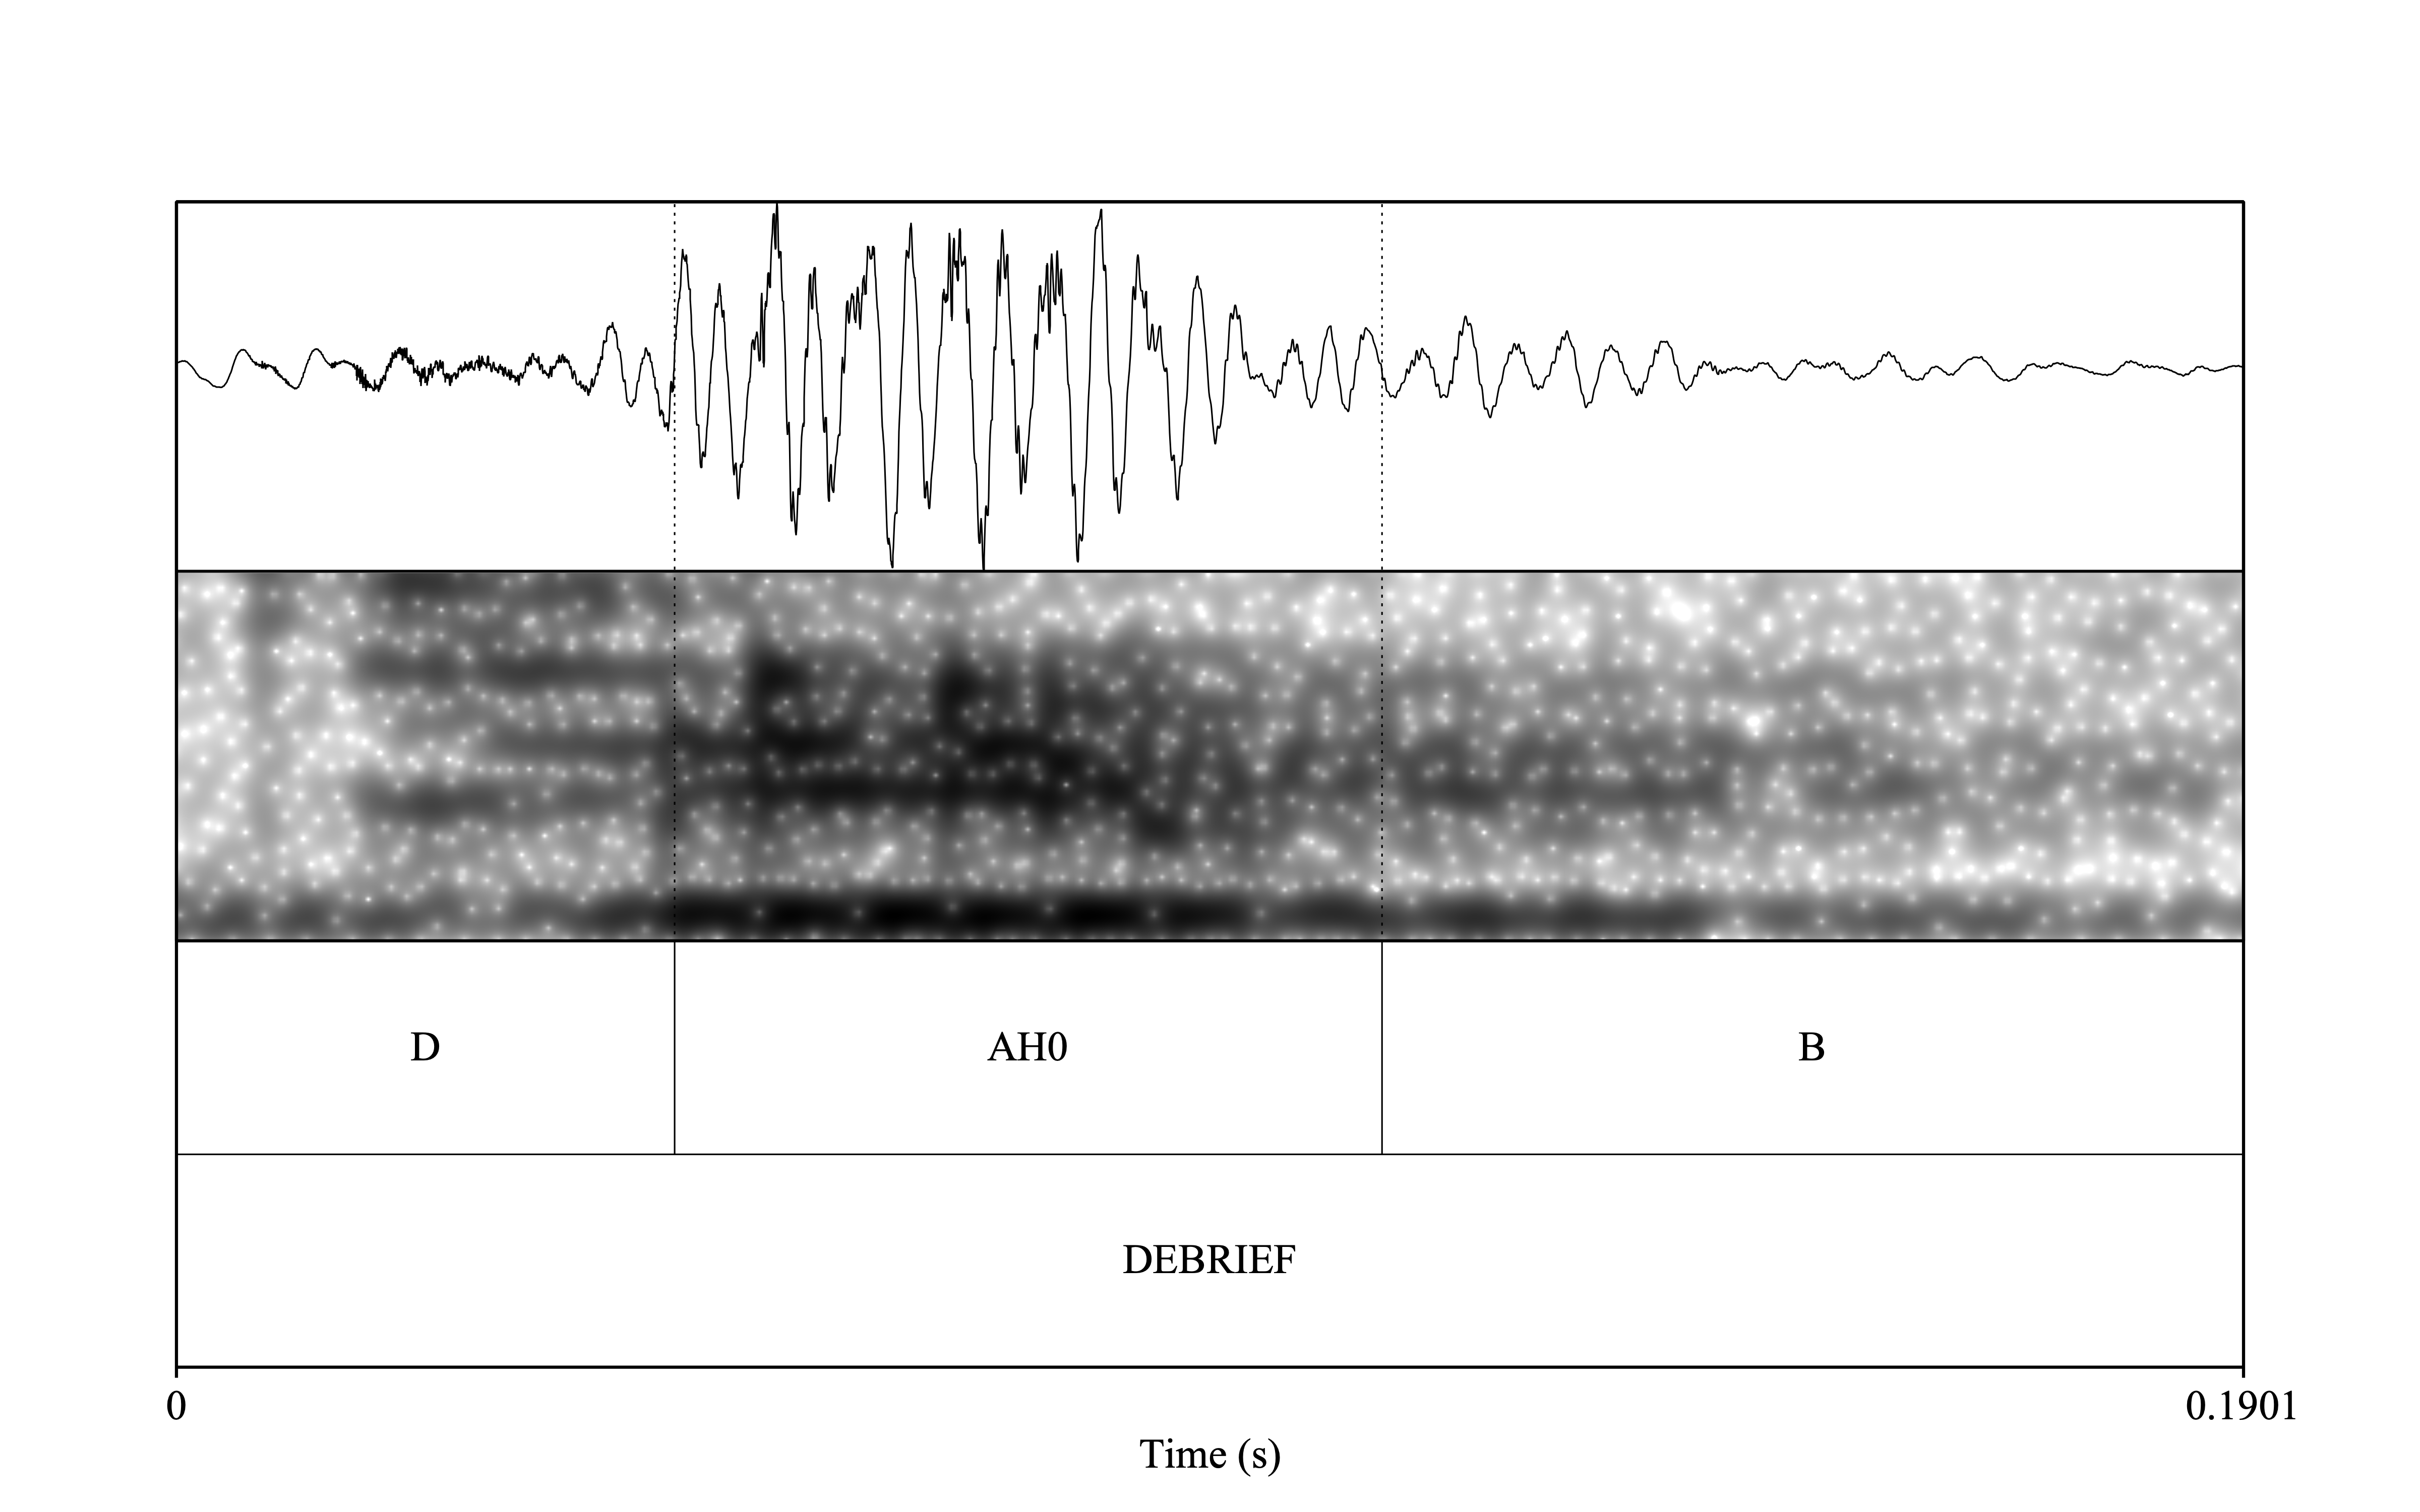
\includegraphics[width=\textwidth]{figures/gutierrez_deb_600.png}
    \caption{A portion of the waveform and spectrogram for the word ``debrief.'' There is no clear burst in the waveform or spectrogram, indicating an approximant-like production. The [ð]-like production was confirmed by the audio.}
    \label{fig:gutierrez:debriefing}
\end{figure}

The acoustic measurements for each token were obtained automatically from the aforementioned 20ms burst window using the same script. For the spectral analysis, the spectral shape of the burst was calculated from the burst window alone using basic Praat functions. The \textsc{ri} was calculated by subtracting the intensity from the burst window from the intensity from the following vowel. The values from each of the five acoustic properties were submitted to one of five mixed-effects linear regression models -- one model per measurement. The models were created in R using the lmerTest package \citep{r,lmer}. Each model included the continuous dependent variable as a function of the interaction of \textsc{language} (English, Spanish) with three lexical factors: \textsc{frequency} (high, low), \textsc{vocabulary} (IT, non-IT), and \textsc{cognate} (cognate, non-cognate) status. Additionally, \textsc{word} and \textsc{participant} were included as random variables. See \ref{ex:gutierrez:stats_model} for an illustration of the models.

\begin{enumerate}
    \item\label{ex:gutierrez:stats_model} model = lmer(DV $\sim$ Lang \textasteriskcentered{} Freq + Lang \textasteriskcentered{} Vocab + Lang \textasteriskcentered{} Cognate + (1|word) + (1|Participant)
\end{enumerate}

\section{Results}\label{sec:gutierrez:results}

\subsection{Spectral measurements}

All four models report a difference in spectral shape (i.e. energy distribution of the burst) between Spanish and English tokens (\textit{p} \textless{} 0.001). While English bursts had higher values of \textsc{cog} and \textsc{sd}, Spanish had higher values of skewness and kurtosis. A summary of general results is provided in \tabref{tab:gutierrez:cog_results} (only significant results are reported).  Plots of the four spectral moments, presented by language, are shown in \figref{fig:gutierrez:spec4}. Furthermore, there was an interaction between \textsc{language} and \textsc{vocabulary}, where Spanish non-IT words had lower values for skewness and kurtosis, relative to English IT words (\textit{p} \textless{} 0.031 and \textit{p} \textless{} 0.025, respectively). That is, Spanish non-IT lexical items had skewness and kurtosis values that were more Spanish-like, relative to the more alveolar-like English IT words. The models did not return any other significant main effects or interactions between language and the linguistic factors under examination (i.e. lexical frequency category and cognate status).

\begin{table}
\caption{Summary of spectral shape results, separated by model.}
\label{tab:gutierrez:cog_results}
 \begin{tabular}{llrrrr}
 \lsptoprule
 Model & & Estimate & Std. error & \textit{p}-value &  \\
 \midrule
 \multirow{2}{*}{\textsc{cog}} & (Intercept) & 1.051e+03 & 1.420e+02 & 2.28e-06 & *** \\
 & Lang\_Spanish & -5.376e+02 & 9.252e+01 & 3.21e-08 & *** \\
 \addlinespace[2ex]
 \multirow{2}{*}{\textsc{sd}} & (Intercept) & 1607.343 & 199.131 & 3.27e-06 & *** \\
 & Lang\_Spanish & -680.513 & 90.7111 & 3.38e-12 & *** \\
 \addlinespace[2ex]
 \multirow{3}{*}{Skewness} & (Intercept) & 9.10204 & 1.72910 & 0.000253 & *** \\
 & Lang\_Spanish & 3.90179 & 0.60039 & 8.97e-10 & *** \\
 & Lang\_Sp:Vocab\_non-IT & -1.48964 & 0.68651 & 0.031 & * \\
 \addlinespace[2ex]
 \multirow{3}{*}{Kurtosis} & (Intercept) & 184.038 & 71.024 & 0.0243 & * \\
 & Lang\_Spanish & 157.351 & 27.862 & 6.89e-08 & *** \\
 & Lang\_Sp:Vocab\_non-IT & -72.084 & 31.869 & 0.0250 & * \\
 \lspbottomrule
 \end{tabular}
\end{table}

All in all, the results for \textsc{cog}, \textsc{sd}, skewness and kurtosis indicate that these Spanish--L1--English--L2 bilingual speakers produce acoustic properties in their speech that differ as a function of language. That is to say, the distribution of these values varies depending on the language the speakers are using. Given that these measurements have been reported as indicative of \textsc{poa}, these results can be interpreted as indicating that these bilinguals have an alveolar-like (i.e. more English-like) production of /d/ in English and a dental-like (i.e. more Spanish-like) articulation of /d̪/ in their Spanish speech. Burst productions do not appear to be influenced by other factors such as lexical frequency category or cognate status.

\begin{figure}
    
    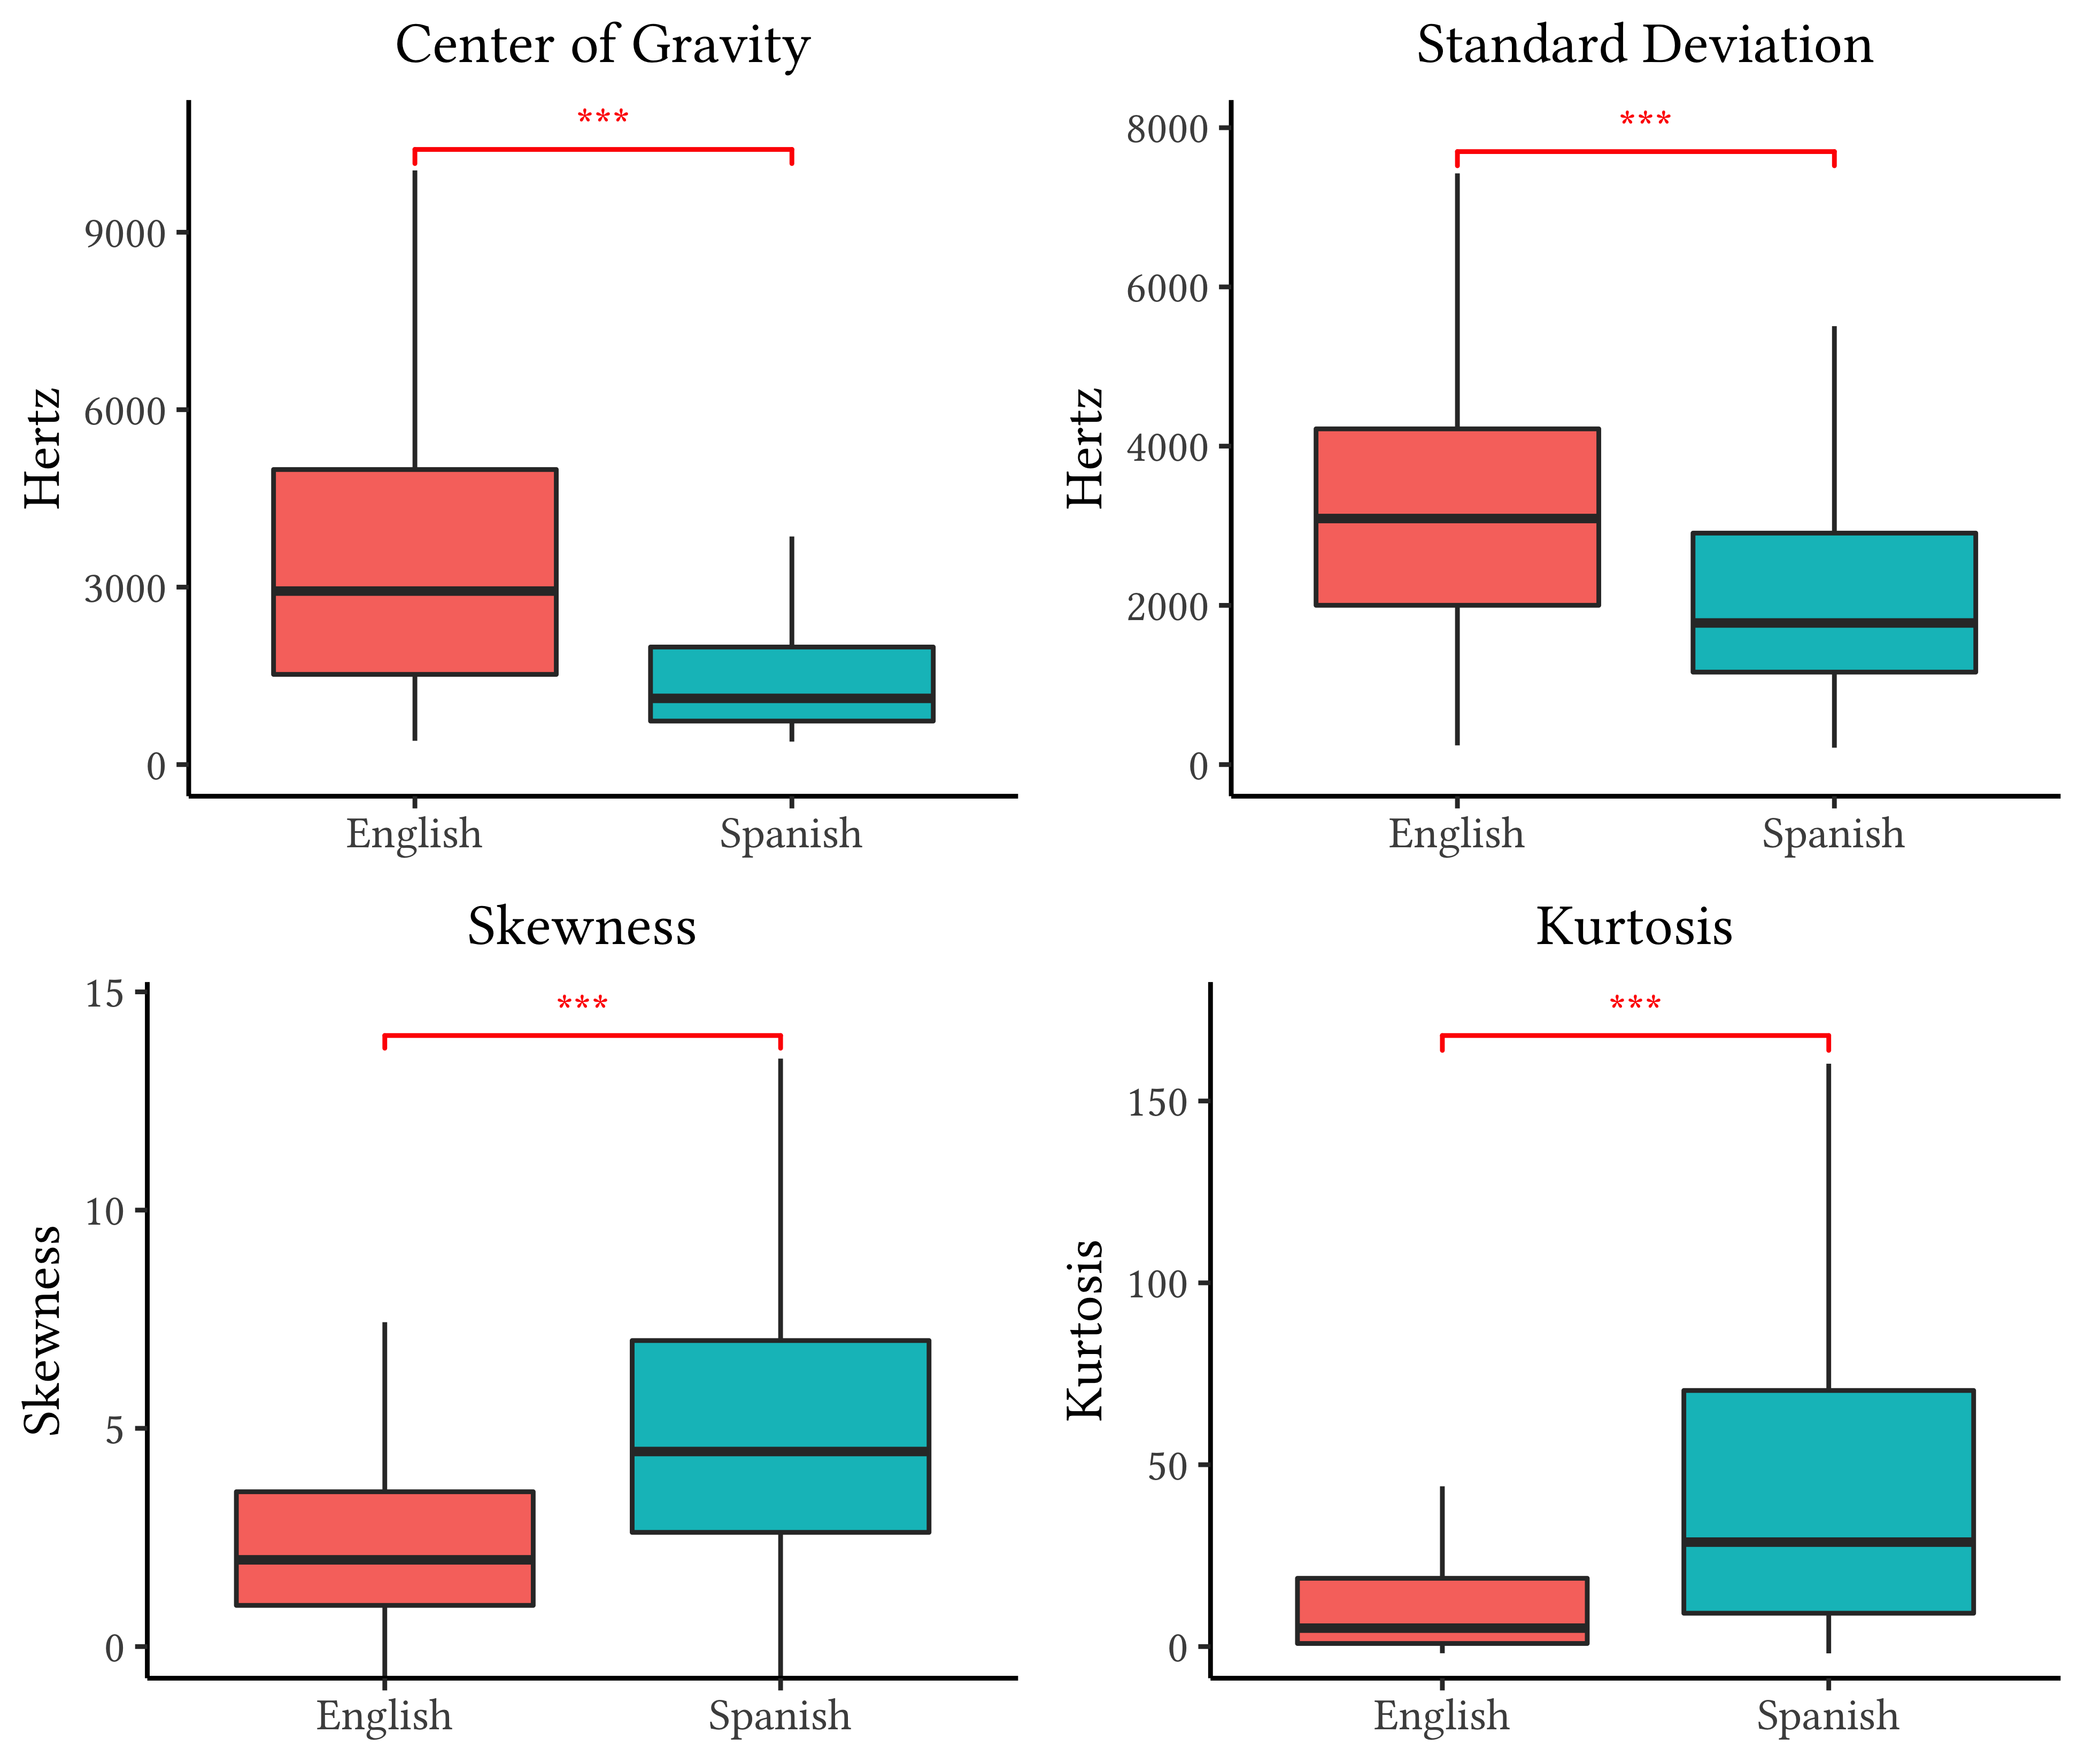
\includegraphics[width=\textwidth]{figures/gutierrez_4spec_plot.png}
    \caption{Spectral measurements. The distribution of values for all four spectral moments varied as a function of language.}
    \label{fig:gutierrez:spec4}
\end{figure}

\subsection{Relative intensity}

Similar to spectral measurements, \textsc{ri} also returned a main effect of \textsc{language} (\textit{p} \textless{} 0.001). Spanish stops in these data have a higher \textsc{ri} than English stops (see \figref{fig:gutierrez:ri_lang}). There was also a main effect of \textsc{vocabulary} (\textit{p} \textless{} 0.014), along an interaction of \textsc{language} ∗ \textsc{vocabulary} (\textit{p} = 0.015). Significant results for relative intensity are reported in \tabref{tab:gutierrez:ri_results}. A post-hoc analysis showed that, only in English, a vocabulary effect occurred; more precisely, IT lexicon in English had a more alveolar-like production (i.e. lower \textsc{ri}) than general English vocabulary (\textit{p} = 0.015). This interaction is presented in \figref{fig:gutierrez:ri_vocab}. Spanish productions did not differ as a function of vocabulary status (\textit{p} = 0.78).

\begin{table}
\caption{Summary of relative intensity results.}
\label{tab:gutierrez:ri_results}
 \begin{tabular}{lrrrr}
 \lsptoprule
 & Estimate & Std. Error & \textit{p}-value &  \\
 \midrule
 (Intercept) & -6.5241 & 0.6053 & 1.99e-12 & *** \\
 Lang\_Spanish & 3.1740 & 0.6089 & 5.03e-07 & *** \\
 CogStatus\_Non-cog & -0.9627 & 0.4456 & 0.0324 & * \\
 Vocab\_non-IT & 1.1198 & 0.4480 & 0.1350 & * \\
 Lang\_Sp:Vocab\_non-IT & -1.7019 & 0.6951 & 0.0153 & * \\
 \lspbottomrule
 \end{tabular}
\end{table}

\begin{figure}
    \subfigure[\textsc{ri} by language]{{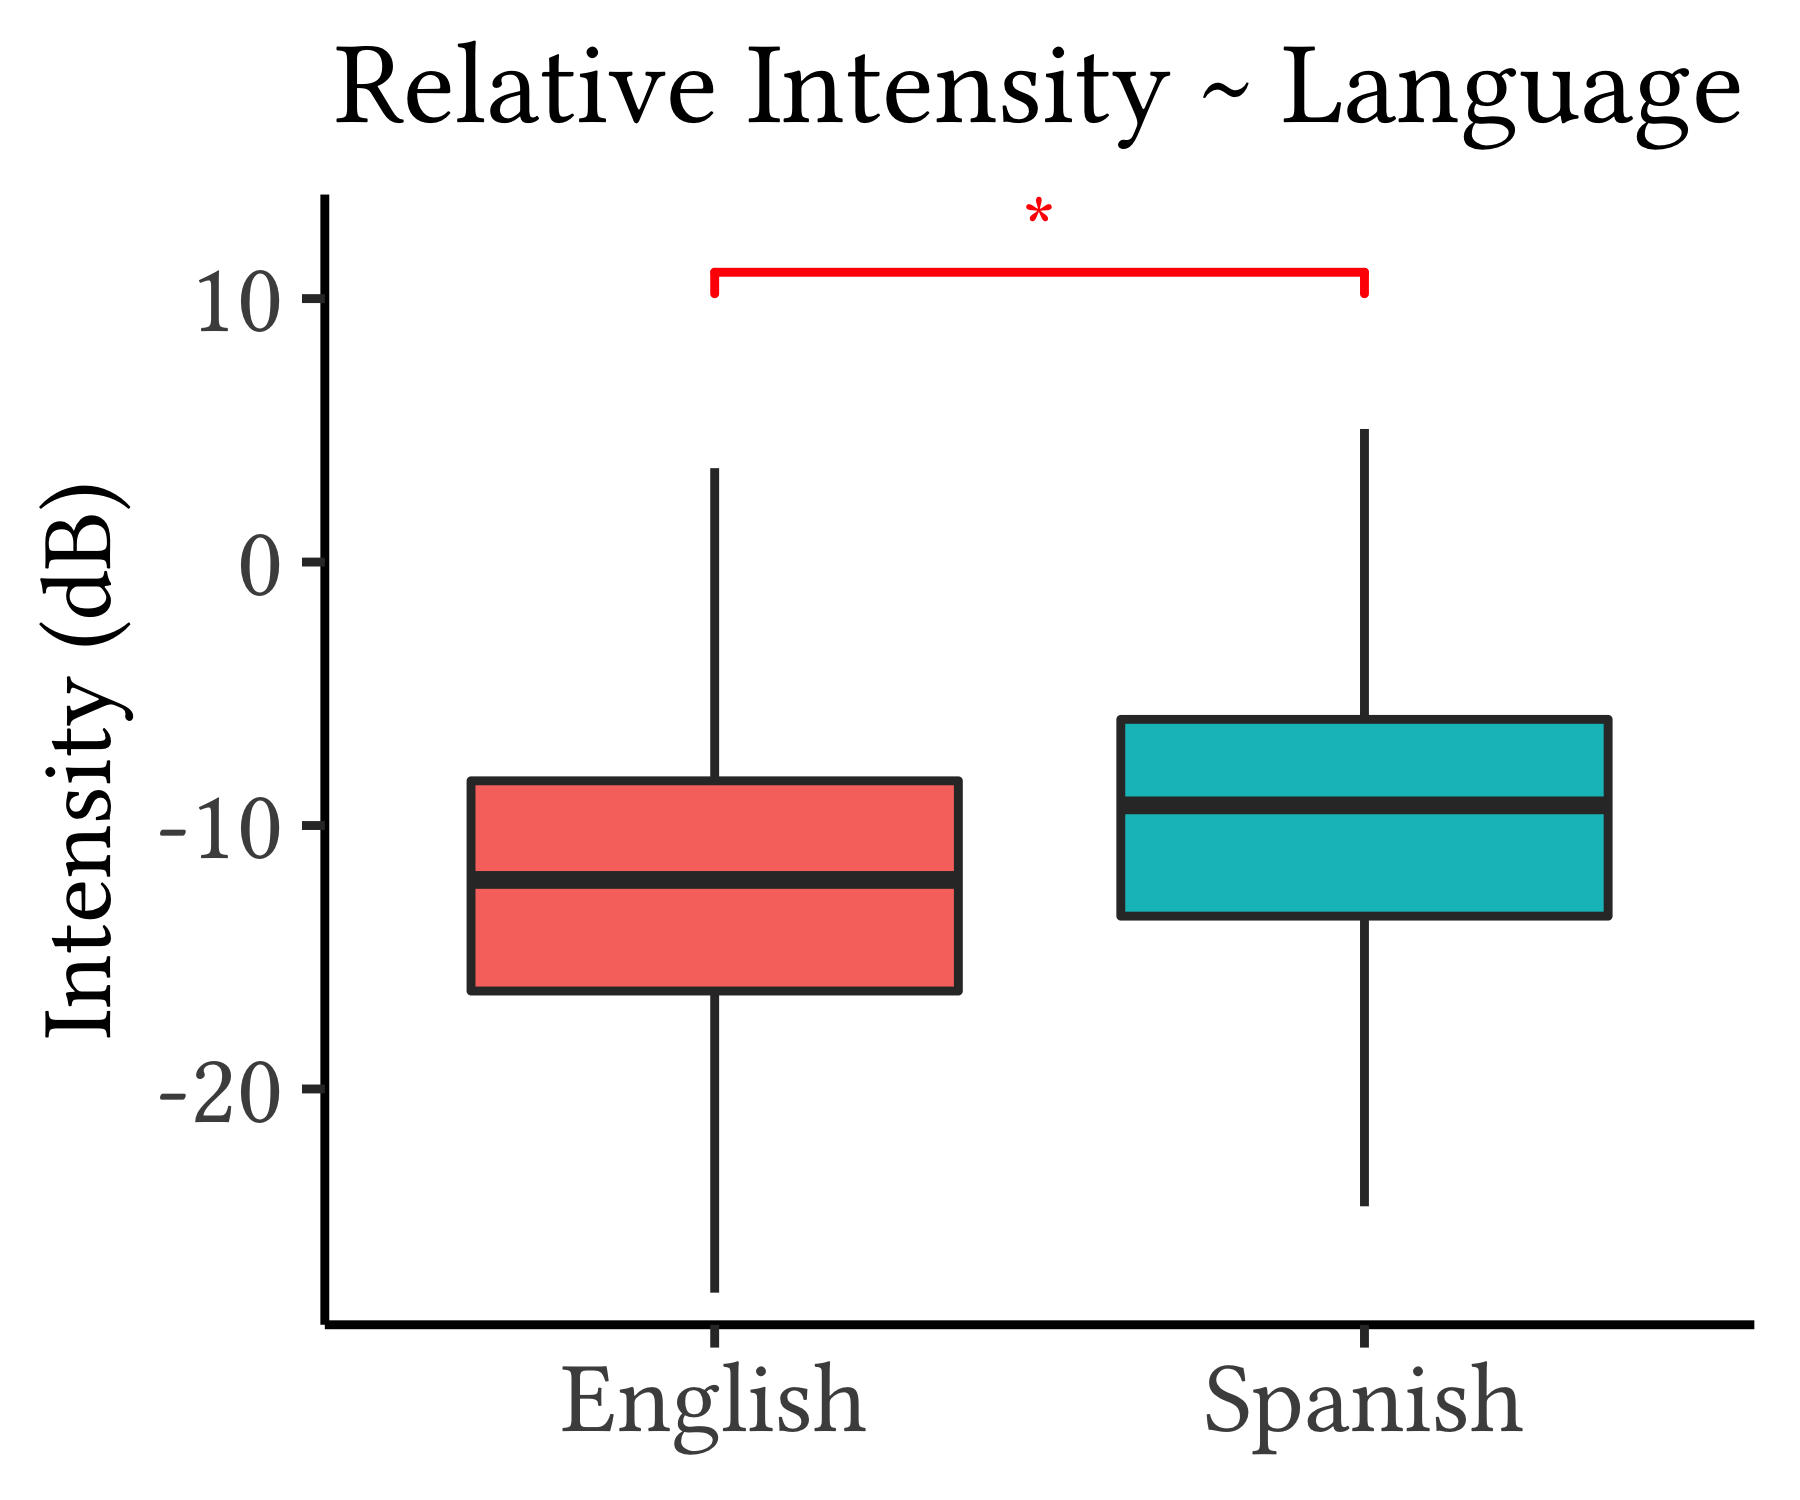
\includegraphics[height=1.71in]{figures/gutierrez_RI_lang.png} \label{fig:gutierrez:ri_lang} }}%
    \qquad
    \subfigure[ \textsc{ri} by vocab status]{{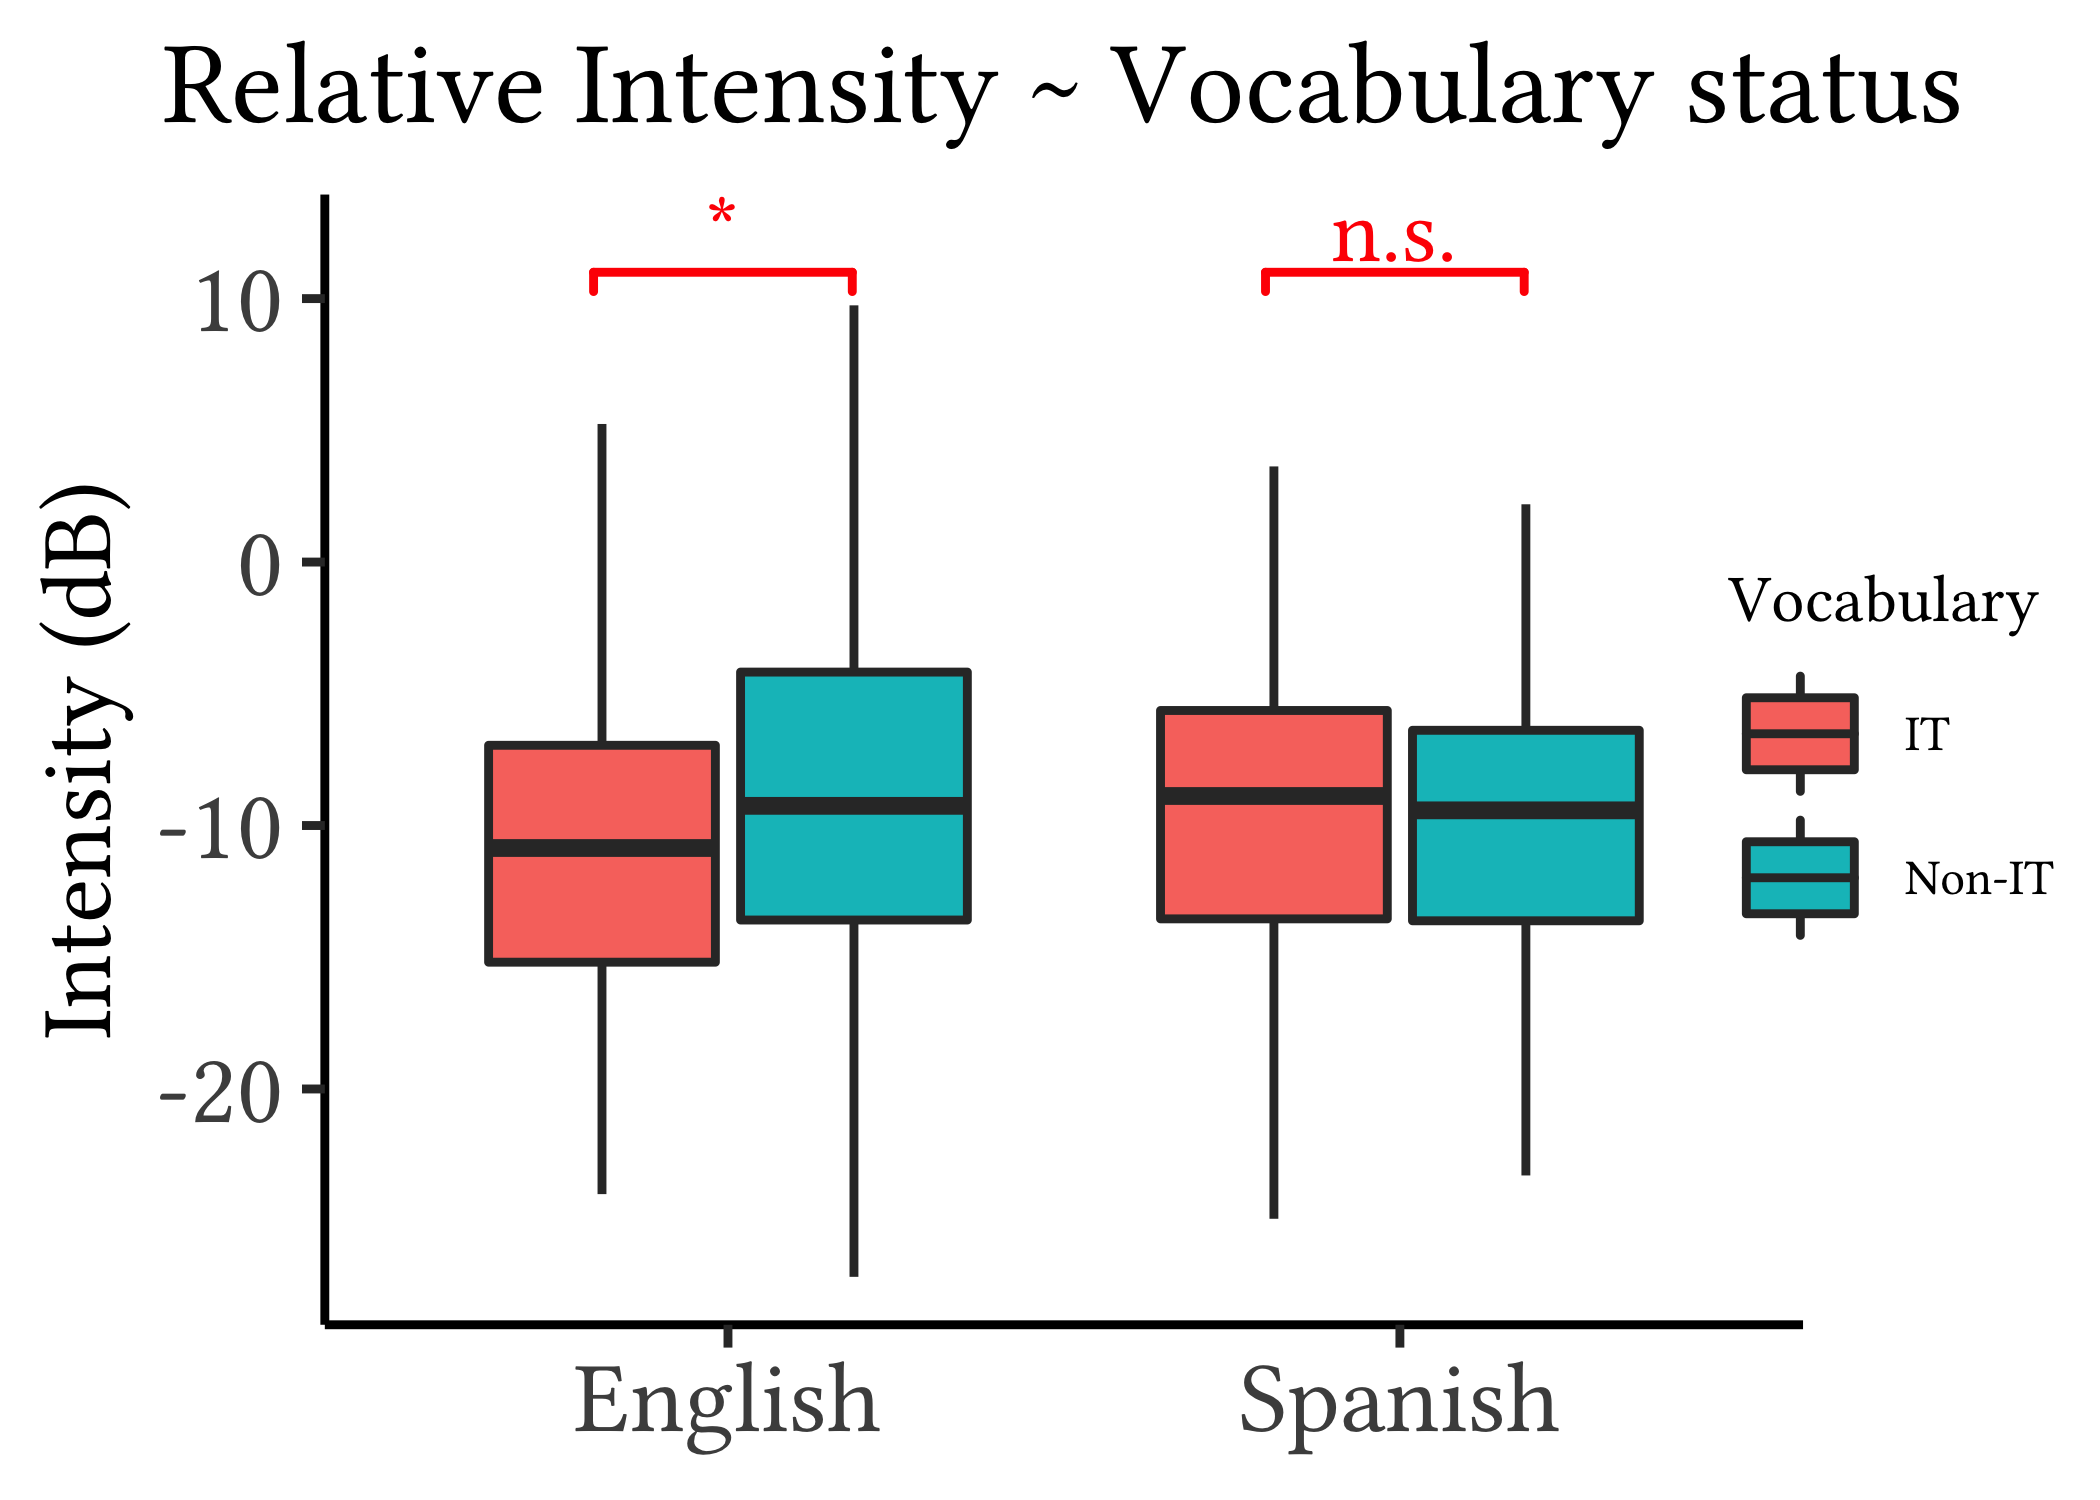
\includegraphics[height=1.71in]{figures/gutierrez_RI_vocab.png} \label{fig:gutierrez:ri_vocab} }}%
    \caption{Relative Intensity distributions across language and vocabulary status.}%
    \label{fig:gutierrez:ri_graphs}%
\end{figure}

In the \textsc{language} interaction with \textsc{vocabulary} (refer to \figref{fig:gutierrez:ri_vocab}), in English, CPS status has an effect on the production of /d/. Words in the IT lexicon  have a lower \textsc{ri}; that is, they are more English-like. Words that are part of the general domain (i.e. general vocabulary) have a higher \textsc{ri}; that is, they are more Spanish-like. This signals that the words related to the speakers' profession and the ones they are constantly using in English have a more alveolar-like production.

\section{Discussion}\label{sec:gutierrez:discussion}

To summarize the results presented above, \textsc{cog}, \textsc{sd}, skewness, kurtosis, and \textsc{ri} all showed a distinction in the energy distribution between English and Spanish voiced coronal stop burst of bilingual speakers. Moreover, models of skewness, kurtosis, and \textsc{ri} also report an interaction between \textsc{language} and \textsc{vocabulary}, where English IT words were more alveolar-like and Spanish non-IT lexical items were more dental-like. Lastly, the \textsc{ri} statistical model also returned main effects of \textsc{cognate} status and \textsc{vocabulary}, indicating that English IT words as well as English non-cognate words were more alveolar-like than their respective Spanish counterparts, corroborating the hypotheses stated above.

Because these five acoustic cues are reported to be indicative of \textsc{poa}, the results regarding the main effect of \textsc{language} in all five metrics suggest that the participants have two articulations. That is, they have an articulation for English (i.e. [d] or more alveolar-like productions) and another for Spanish (i.e. [d̪] or more dental-like productions). Although \textsc{ri} results showed an interaction between the two \textsc{vocabulary} levels in English data, no such interaction was observed in Spanish words. General English vocabulary did not differ in \textsc{ri} values from Spanish IT or Spanish general lexicon (refer back to \figref{fig:gutierrez:ri_vocab}). To exemplify this finding, these data indicate that words such as \textit{directory} and \textit{debug} are produced with acoustics that are more alveolar-like than the acoustics for words such as \textit{decline} or \textit{debilitate}. The acoustics in the latter pair tend to pattern similarly to Spanish words.

In a study of Canadian-English--Canadian-French bilinguals, \citet{sundara2006production} found two phonetic categories in their speakers, as indicated by differences in spectral measurements. The results in the present study are indicative of a generalizable pattern in languages such as the Romance Languages (i.e. languages with a dental articulation) and English. The linguistic pattern under discussion is a bimodal articulation of coronal stops; Mexican-Spanish--American-English as well as Canadian-English--Canadian-French bilinguals have an alveolar /d/ in English and a dental /d̪/ in the other language. In other words, acoustic differences suggest that there are two phonetic representations; but it is unclear if, in this present study, these representations are Spanish-monolingual-like and English-monolingual-like. To make this determination, acoustic properties of the /d/ produced by Spanish--English bilinguals need to be compared to those produced by Spanish and English monolinguals under similar conditions.

Usage-based models, as described by \citeauthor{bybee2001phonology}, postulate that the form and content of sound systems are shaped by language exposure and usage. ``In particular, the frequency with which individual words ... are used and the frequency with which certain patterns recur in a language affects the nature of mental representation and in some cases the actual phonetic shape of words'' (\citeyear[1]{bybee2001phonology}). Given the results from all five acoustic metrics analyzed in the present study, the bilingual speakers demonstrated one phonetic category per language -- there is a main effect of language in all metrics. Additionally, as suggested by skewness, kurtosis, and \textsc{ri} results, considering the bilingual context in which these speakers interact with their two languages, the creation or development of a phonetic (articulatory) category in their L2 sound system appears to be governed by the heightened exposure to and usage of a specific type of CPS lexicon: IT vocabulary.

On the one hand, it is evident that \textsc{frequency} type (high- vs low-frequency) was unable to predict the energy distribution in voiced coronal stop bursts for these data. On the other hand, \textsc{vocabulary} status interacted with \textsc{language} as reported for skewness, kurtosis, and \textsc{ri}. Referring back to \tabref{tab:gutierrez:stimuli}, we can see that some IT words such as \textit{directory} and \textit{debug} are coded as low-frequency in accordance with general lexical frequency sources such as the NIM corpora. Nonetheless, it goes without saying that these and many other terms that were labeled as low-frequency are, in fact, commonplace in the IT lexicon of coders or software developers. As demonstrated by the results in this study, vocabulary status was able to account for some of the variation present in the productions by these bilingual speakers, while lexical frequency was not. For that reason, I take these results as evidence of lexical effects at the level of the community of practice. As such, I advocate for the usage of Community of Practice-Specific (CPS) lexicon, instead of general vocabulary, when studying the lexical frequency effects in language variation. This suggested approach goes beyond the previously implemented `local frequency' used in studies such as \citet{erker2012role}, \citet{file2011gradient}, and \citet{linford2013lexical}. 

The incorporation of CPS lexicon in this study was done to re-evaluate traditional frequency norms. In psycholinguistic research, lexical frequency is typically determined by population-general language use. In more recent production studies, the local frequencies approximate the trends in natural language usage by the speech community. However, even this approach obscures the fact that these corpora from which the local frequencies are obtained may include members from different communities of practice who will likely have distinct linguistic behaviors. Furthermore, population-general frequencies, when obtained from all sectors of the population, are an aggregate of different registers and dialects from many communities -- or even countries, as is the case with NIM's corpora. On the other hand, lexical frequencies that are based on CPS linguistic patterns will be more centered around the speaker's experience. That is, a corpus -- or even a word list -- that is obtained from the linguistic practices common in the environment in which the individual is immersed in on a daily basis will be more characteristic of the speaker's language exposure and language use. This study, in fact, shows a lexical effect of CPS vocabulary status, where the acquisition of a new phonetic category (i.e. an alveolar [d]) appears to be mediated by the heightened-frequency CPS lexicon (i.e. terminology that the participants in this study have high exposure to on a daily basis).

An equally important finding from the present study is the successful data collection approach introduced here. As a reminder, from the 224 tokens that were discarded from this study, 173 (or more than 77\%) of these cases were due to approximant-like productions that lacked a burst. Less than 21\% ($n$ = 47) of these tokens were discarded due to poor audio quality. This indicates that remote data collection that relies on the execution of self-recordings by the participants themselves is a feasible approach that is able to yield high quality audio recordings for phonetic research. This is of paramount significance in the present day, considering the public health crisis that is taking place worldwide as a result of COVID-19. This methodology may allow speech researchers to continue acoustic analyses without violating local, state, and federal mandates and restrictions and without endangering public health. In the long-term, this approach may also be used for data collection with populations around the world when travel advisories, funding limitations, etc. may not permit direct access to those communities. An important caveat, however, is the kinds of populations that this approach may be implemented with. For example, accessibility to the internet and other technological resources, as well as familiarity with these resources by the participants is necessary for such a data collection approach. For this study, I was able to collect data remotely because my participants had access to the internet and to a computer, and they knew how to use them without the need for additional training. This will not be the case for every community, and certainly not for every age group.

In sum, Community of Practice-Specific lexicon, as indicated by these results, is a better predictor for frequency effects than population-general norms. I argue that finding a CPS lexicon that is associated with groups of interest for linguists (e.g. professional, social, regional, etc.) will be more useful and fruitful in approximating high-exposure, and thus high-frequency, lexicon. Moreover, these results contribute to the assertion of the generalization for a bimodal articulation of [d $\sim$ d̪] (and perhaps [t $\sim$ t̪]) in bilingual speakers of alveolar- and dental-stop languages.

\section{Conclusion}\label{sec:gutierrez:conclusion}

In this paper, I explored the production of coronal stops by early Spanish–English bilinguals. The present study found that bilinguals have two articulatory categories, as the acoustic properties of their speech in both languages demonstrate. I also report that Community of Practice-Specific status (that is, IT vocabulary) is more likely to predict articulatory variation, and thus the creation of a new phonetic category. All in all, the present study expands our understanding of bilingual speech and provides novel methodological approaches for (sociophonetic) research studies. On the basis of these results and the present methodology, future studies may explore the production of voiced and voiceless coronal stops as articulated by other (Spanish–English) bilingual populations, paying attention to the CPS lexicon; may further our understanding of the perception of coronal stops \citep[e.g.][]{melguy2018exploring}; or may even trace the gestural trajectory of the articulators with imaging technology to obtain the precise place of articulation for coronal sounds. Additionally, future studies may adopt the remote data collection methodology presented here, with modifications where necessary.

\section*{Acknowledgements}
I am grateful to Dr. Justin Davidson and Dr. Susan Lin for their assistance and guidance in the development of this project idea and methodology. I also want to thank two anonymous reviewers, in addition to Dr. Davidson, Dr. Lin, and Annie Helms, for their invaluable feedback and suggestions for improvement of previous drafts of this manuscript. Most importantly, I want to acknowledge and thank my participants for lending their voices to my study. This project was made possible thanks to the Graduate Dean's Summer Research Grant from UC Berkeley.

\printbibliography[heading=subbibliography,notkeyword=this]

\end{document}